
%(BEGIN_QUESTION)
% Copyright 2010, Tony R. Kuphaldt, released under the Creative Commons Attribution License (v 1.0)
% This means you may do almost anything with this work of mine, so long as you give me proper credit

Some programmable logic controllers (PLCs) do not have a built-in PID instruction, and so to implement PID control in one of these PLCs the technician or engineer must build their own PID algorithm from math statements.  Examine this ladder-logic program for a PLC implementing full PID control:

$$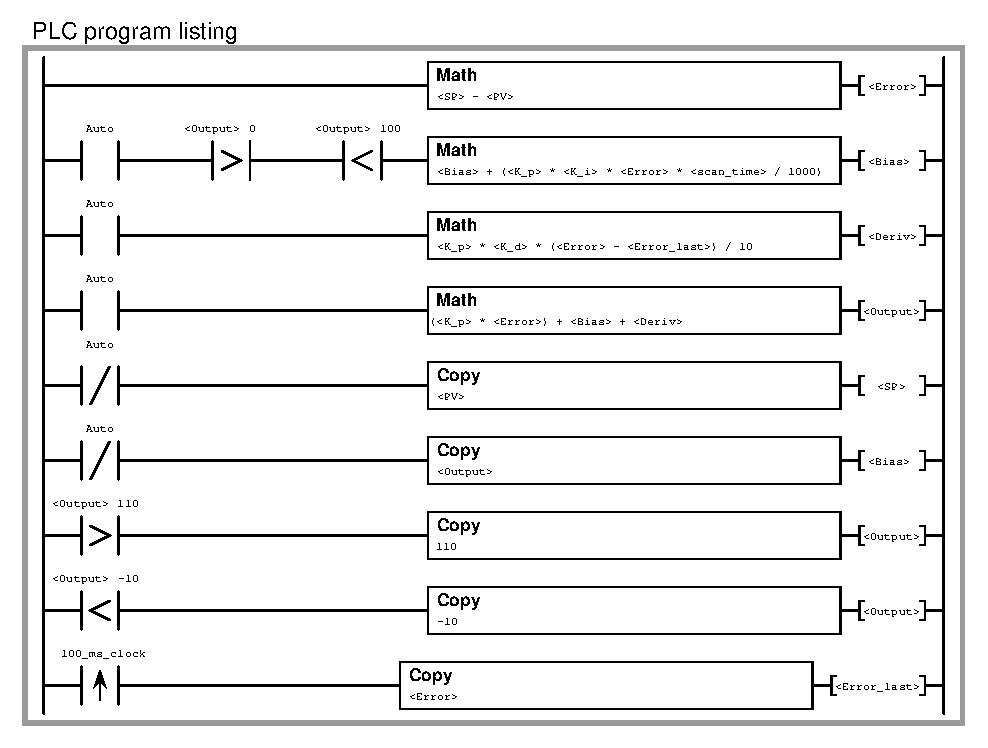
\includegraphics[width=15.5cm]{i02674x01.eps}$$

\begin{itemize}
\item{} Is this a {\it direct-acting} or a {\it reverse-acting} algorithm?  Which instruction(s) in the program indicate this?
\vskip 5pt
\item{} Does this program implement the {\it Parallel}, {\it Ideal}, or {\it Series} PID equation?  Which instruction(s) in the program indicate this?  
\vskip 5pt
\item{} Where does the program implement the feature of {\it setpoint tracking}?
\vskip 5pt
\item{} Where does the program implement the feature of {\it output tracking}?
\vskip 5pt
\item{} Where is integral action (I) calculated in this program?
\end{itemize}

\vskip 20pt \vbox{\hrule \hbox{\strut \vrule{} {\bf Suggestions for Socratic discussion} \vrule} \hrule}

\begin{itemize}
\item{} Modify this PLC program so that it implements the {\it other} direction of action (i.e. reverse-action instead of direct-action, or vice-versa).
\item{} Modify this PLC program so that it implements a different PID equation from the one it implements now.
\item{} Modify this PLC program so that it implements a P+I equation (no derivative).
\item{} Modify this PLC program so that it implements a P+D equation (no integral).
\item{} Modify this PLC program so that it implements an I+D equation (no proportional).
\item{} What is the significance of the ``$\uparrow$'' symbol inside the 100\_ms\_clock contact?
\item{} What is the significance of each ``$<$'' and ``$>$'' symbol inside some of the contacts?
\item{} Where does this program implement {\it reset windup limiting}?
\item{} Would it make any difference if the Error\_last ``copy'' instruction were placed at the beginning of the program instead of the very end of the program?  Hint: consider when a PLC typically scans its I/O to update any discrete and analog values -- in the portion of the execution cycle {\it outside} the program scan.
\end{itemize}

\underbar{file i02674}
%(END_QUESTION)





%(BEGIN_ANSWER)


%(END_ANSWER)





%(BEGIN_NOTES)

\begin{itemize}
\item{} Is this a {\it direct-acting} or a {\it reverse-acting} algorithm?  Which instruction(s) in the program indicate this? {\it The first rung, where Error is calculated, defines this as a reverse-acting controller (Error = SP $-$ PV).}
\vskip 10pt
\item{} Does this program implement the {\it Parallel}, {\it Ideal}, or {\it Series} PID equation?  Which instruction(s) in the program indicate this?  {\it The equation used here is the Ideal, and we know this because both the Bias and Derivative calculations incorporate the gain constant (K\_p).}
\vskip 10pt
\item{} Where does the program implement the feature of {\it setpoint tracking}?  {\it In the ``copy'' instruction where SP is set equal to PV when the controller is in manual mode.}
\vskip 10pt
\item{} Where does the program implement the feature of {\it output tracking}?  {\it In the ``copy'' instruction where Bias is set equal to Output when the controller is in manual mode.}
\vskip 10pt
\item{} Where is integral action (I) calculated in this program?  {\it Integral action is actually calculated as ``Bias'', where that value accumulates error-time product in automatic mode.  In manual mode, the Bias value is set equal to the output, and error goes to zero due to setpoint tracking.}
\end{itemize}

%INDEX% Control, proportional + integral + derivative: PLC program
%INDEX% PLC, demonstration program: PID control algorithm

%(END_NOTES)


